% generated by Plantuml 1.2025.4       
\definecolor{plantucolor0000}{RGB}{255,255,255}
\definecolor{plantucolor0001}{RGB}{0,0,0}
\definecolor{plantucolor0002}{RGB}{194,194,194}
\definecolor{plantucolor0003}{RGB}{24,24,24}
\definecolor{plantucolor0004}{RGB}{84,84,84}
\definecolor{plantucolor0005}{RGB}{166,166,166}
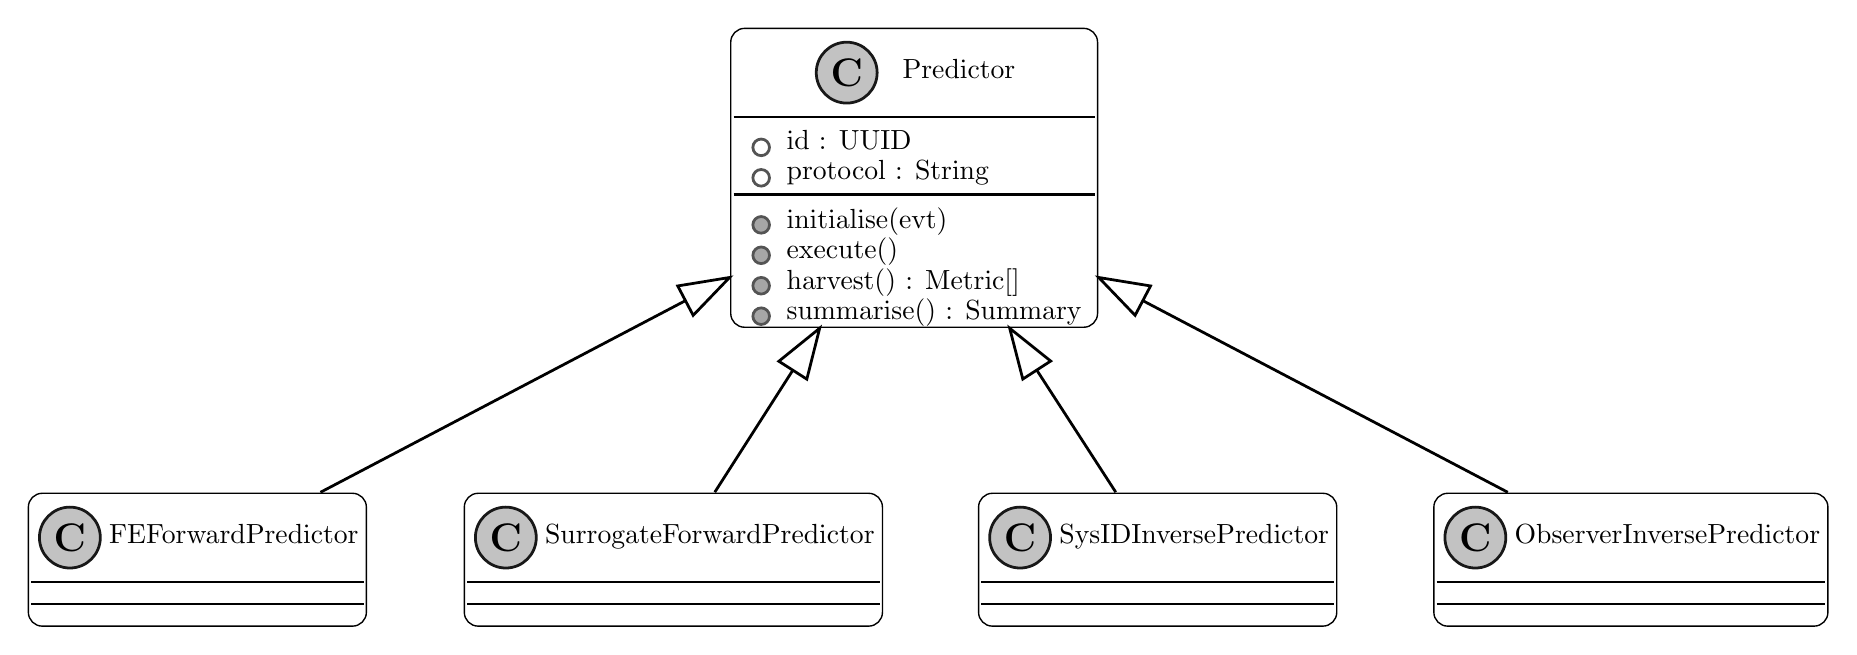
\begin{tikzpicture}[yscale=-1
,pstyle0/.style={color=black,fill=white,line width=0.5pt}
,pstyle1/.style={color=plantucolor0003,fill=plantucolor0002,line width=1.0pt}
,pstyle2/.style={color=black,line width=0.5pt}
,pstyle3/.style={color=plantucolor0004,line width=1.0pt}
,pstyle4/.style={color=black,line width=1.0pt}
,pstyle5/.style={color=plantucolor0004,fill=plantucolor0005,line width=1.0pt}
]
\draw[pstyle0] (260.8pt,12pt) arc (180:270:5pt) -- (265.8pt,7pt) -- (388.35pt,7pt) arc (270:360:5pt) -- (393.35pt,12pt) -- (393.35pt,110pt) arc (0:90:5pt) -- (388.35pt,115pt) -- (265.8pt,115pt) arc (90:180:5pt) -- (260.8pt,110pt) -- cycle;
\draw[pstyle1] (302.7055pt,23pt) ellipse (11pt and 11pt);
\node at (302.7055pt,23pt)[]{\textbf{\Large C}};
\node at (322.6845pt,18pt)[below right,color=black,inner sep=0]{Predictor};
\draw[pstyle2] (261.8pt,39pt) -- (392.35pt,39pt);
\draw[pstyle3] (271.8pt,50pt) ellipse (3pt and 3pt);
\node at (280.8pt,43.5pt)[below right,color=black,inner sep=0]{id : UUID};
\draw[pstyle3] (271.8pt,61pt) ellipse (3pt and 3pt);
\node at (280.8pt,54.5pt)[below right,color=black,inner sep=0]{protocol : String};
\draw[pstyle4] (261.8pt,67pt) -- (392.35pt,67pt);
\draw[pstyle5] (271.8pt,78pt) ellipse (3pt and 3pt);
\node at (280.8pt,71.5pt)[below right,color=black,inner sep=0]{initialise(evt)};
\draw[pstyle5] (271.8pt,89pt) ellipse (3pt and 3pt);
\node at (280.8pt,82.5pt)[below right,color=black,inner sep=0]{execute()};
\draw[pstyle5] (271.8pt,100pt) ellipse (3pt and 3pt);
\node at (280.8pt,93.5pt)[below right,color=black,inner sep=0]{harvest() : Metric[]};
\draw[pstyle5] (271.8pt,111pt) ellipse (3pt and 3pt);
\node at (280.8pt,104.5pt)[below right,color=black,inner sep=0]{summarise() : Summary};
\draw[pstyle0] (7pt,180pt) arc (180:270:5pt) -- (12pt,175pt) -- (124.14pt,175pt) arc (270:360:5pt) -- (129.14pt,180pt) -- (129.14pt,218pt) arc (0:90:5pt) -- (124.14pt,223pt) -- (12pt,223pt) arc (90:180:5pt) -- (7pt,218pt) -- cycle;
\draw[pstyle1] (22pt,191pt) ellipse (11pt and 11pt);
\node at (22pt,191pt)[]{\textbf{\Large C}};
\node at (36pt,186pt)[below right,color=black,inner sep=0]{FEForwardPredictor};
\draw[pstyle2] (8pt,207pt) -- (128.14pt,207pt);
\draw[pstyle2] (8pt,215pt) -- (128.14pt,215pt);
\draw[pstyle0] (164.53pt,180pt) arc (180:270:5pt) -- (169.53pt,175pt) -- (310.62pt,175pt) arc (270:360:5pt) -- (315.62pt,180pt) -- (315.62pt,218pt) arc (0:90:5pt) -- (310.62pt,223pt) -- (169.53pt,223pt) arc (90:180:5pt) -- (164.53pt,218pt) -- cycle;
\draw[pstyle1] (179.53pt,191pt) ellipse (11pt and 11pt);
\node at (179.53pt,191pt)[]{\textbf{\Large C}};
\node at (193.53pt,186pt)[below right,color=black,inner sep=0]{SurrogateForwardPredictor};
\draw[pstyle2] (165.53pt,207pt) -- (314.62pt,207pt);
\draw[pstyle2] (165.53pt,215pt) -- (314.62pt,215pt);
\draw[pstyle0] (350.36pt,180pt) arc (180:270:5pt) -- (355.36pt,175pt) -- (474.78pt,175pt) arc (270:360:5pt) -- (479.78pt,180pt) -- (479.78pt,218pt) arc (0:90:5pt) -- (474.78pt,223pt) -- (355.36pt,223pt) arc (90:180:5pt) -- (350.36pt,218pt) -- cycle;
\draw[pstyle1] (365.36pt,191pt) ellipse (11pt and 11pt);
\node at (365.36pt,191pt)[]{\textbf{\Large C}};
\node at (379.36pt,186pt)[below right,color=black,inner sep=0]{SysIDInversePredictor};
\draw[pstyle2] (351.36pt,207pt) -- (478.78pt,207pt);
\draw[pstyle2] (351.36pt,215pt) -- (478.78pt,215pt);
\draw[pstyle0] (514.87pt,180pt) arc (180:270:5pt) -- (519.87pt,175pt) -- (652.26pt,175pt) arc (270:360:5pt) -- (657.26pt,180pt) -- (657.26pt,218pt) arc (0:90:5pt) -- (652.26pt,223pt) -- (519.87pt,223pt) arc (90:180:5pt) -- (514.87pt,218pt) -- cycle;
\draw[pstyle1] (529.87pt,191pt) ellipse (11pt and 11pt);
\node at (529.87pt,191pt)[]{\textbf{\Large C}};
\node at (543.87pt,186pt)[below right,color=black,inner sep=0]{ObserverInversePredictor};
\draw[pstyle2] (515.87pt,207pt) -- (656.26pt,207pt);
\draw[pstyle2] (515.87pt,215pt) -- (656.26pt,215pt);
\draw[pstyle4] (244.434pt,105.3893pt) ..controls (197.974pt,129.7893pt) and (153.21pt,153.29pt) .. (112.55pt,174.64pt);
\draw[pstyle4] (260.37pt,97.02pt) -- (241.6443pt,100.0773pt) -- (247.2238pt,110.7013pt) -- (260.37pt,97.02pt) -- cycle;
\draw[pstyle4] (283.24pt,130.5228pt) ..controls (270.1pt,151.0628pt) and (265.46pt,158.31pt) .. (255.04pt,174.6pt);
\draw[pstyle4] (292.94pt,115.36pt) -- (278.1857pt,127.2894pt) -- (288.2942pt,133.7561pt) -- (292.94pt,115.36pt) -- cycle;
\draw[pstyle4] (371.3782pt,130.4725pt) ..controls (384.6682pt,151.0125pt) and (389.39pt,158.31pt) .. (399.93pt,174.6pt);
\draw[pstyle4] (361.6pt,115.36pt) -- (366.3407pt,133.7319pt) -- (376.4157pt,127.2131pt) -- (361.6pt,115.36pt) -- cycle;
\draw[pstyle4] (409.706pt,105.3893pt) ..controls (456.166pt,129.7893pt) and (500.93pt,153.29pt) .. (541.59pt,174.64pt);
\draw[pstyle4] (393.77pt,97.02pt) -- (406.9162pt,110.7013pt) -- (412.4957pt,100.0773pt) -- (393.77pt,97.02pt) -- cycle;
\end{tikzpicture}
